\chapter{Datenschutzgrundverordnung (DSGVO)}
\putz

%Quellen:
%Reis Folien
%https://wirtschaftslexikon.gabler.de/definition/datenschutz-grundverordnung-99476
\section{Aufbau und Inhalt}
\subsection{DSGVO Grundsätze}
Die Datenschutzgrundverordnung\footcite{dsgvo-wiki}, oder im englischen Sprachraum \textbf{General Data Protection Regulation (GDPR)} genannt, soll die Rechte von natürlichen, realen Personen im Bezug auf Verarbeitung deren personenbezogenen Daten, genau definieren und sicherstellen. Die DSGVO wurde am 25. Mai 2016 beschlossen und trat in Kraft. Sie musste ab diesem Zeitpunkt unter Einhaltung einer zwei jährigen Umsetzungsfrist bis 25. Mai 2018 eingehalten werden. Primär soll jedem EU-Bürger das Recht auf informelle Selbstbestimmung garantiert werden und jeder Mensch in der EU soll vor nicht sachgerechter Nutzung der eigenen Daten rechtlich geschützt werden.
Die neue Datenschutz Richtlinie der Europäischen Union ersetzt die bis dahin geltenden \textbf{Datenschutzrichtlinie 95/94}. Das Gesetz wurde als EU Verordnung erlassen und somit in allen Mitgliedsstaaten vollständig übernommen werden. Die Verordnung enthält jedoch 69 sogenannte Öffnungsklauseln, welche den jeweilige Staate der Europäischen Union eine nationale Selbstbestimmung in diese Punkten erlaubt. Zum Beispiel das alter, ab welchem das Gesetz für eine Person gilt. Hier gilt ein Spielraum, dass das Alter, ab wann die DSGVO auf ein Individuum zutrifft, national selbstbestimmt werden kann, jedoch nicht über 16 und nicht unter 13 liegen darf.
%\footnote{https://de.wikipedia.org/wiki/Datenschutz-Grundverordnung}

Artikel 2, der sachliche Anwendungsbereich der DSGVO beinhaltet:
\begin{itemize}
	\item ganz oder teilweise automatisierte Verarbeitung von personenbezogener Daten
	\item manuelle Verarbeitung personenbezogener Daten, welche in einem Dateisystem gespeichert werden
\end{itemize}

Für die Verordnung gibt es gewisse Ausnahmen (Artikel 1, Abs. 2):
\begin{itemize}
	\item im Rahmen von Tätigkeiten, welche nicht in den Anwendungsbereich des Unionsrechts fallen
	\item Tätigkeiten im Rahmen der gemeinsamen Außen- und Sicherheitspolitik (Titel V, Kapitel 2 EUV)
	\item durch natürliche Personen zur Ausübung ausschließlich persönlicher oder familiärer Tätigkeiten
	\item durch die zuständigen Behörden zum Zwecke der Verhütung, Ermittlung, Aufdeckung oder Verfolgung von Straftaten oder der Strafvollstreckung, einschließlich des Schutzes vor und der Abwehr von Gefahren für die öffentliche Sicherheit
\end{itemize}



\subsection{Kapitel und Aufbau der DSGVO}
Die Datenschuttgrundverordnung ist in 11 Kapitel unterteilt. Diese Kapitel sind wiederum in einzelne Artikel unterteile, 99 an der Zahl. Eine Übersicht:

\begin{itemize}
	\item \textbf{Kapitel I (Artikel 1 bis 4)}: Allgemeine Bestimmungen
	\item \textbf{Kapitel II (Artikel 5 bis 11)}: Grundsätze und Rechtmäßigkeit
	\item \textbf{Kapitel III (Artikel 12 bis 23)}: Grundsätze und Rechtmäßigkeit
	\item \textbf{Kapitel IV (Artikel 24 bis 43)}: Verantwortlicher und Auftragsverarbeiter
	\item \textbf{Kapitel V (Artikel 44 bis 50)}: Übermittlungen personenbezogener Daten an Drittländer oder an internationale Organisationen
	\item \textbf{Kapitel VI (Artikel 51 bis 59)}: Unabhängige Aufsichtsbehörden
	\item \textbf{Kapitel VII (Artikel 60 bis 76)}: Zusammenarbeit und Kohärenz, Europäischer Datenschutzausschuss
	\item \textbf{Kapitel VIII (Artikel 77 bis 84)}: Rechtsbehelfe, Haftung und Sanktionen
	\item \textbf{Kapitel IX (Artikel 85 bis 91)}: Vorschriften für besondere Verarbeitungssituationen
	\item \textbf{Kapitel X (Artikel 92 bis 93)}: Delegierte Rechtsakte und Durchführungsrechtsakte
	\item \textbf{Kapitel XI (Artikel 94 bis 99)}: Schlussbestimmungen
\end{itemize}

\subsection{Fachbegriffe}
Bestimmte Fachbegriffe wie "`Verantwortlicher"' oder "`personenbezogene Daten"', sind in der EU Verordnung definiert und beschrieben worden. Hier folgen nun die Definitionen laut Gesetzestext, welche bei Bedarf vereinfacht beschrieben wurden. 

\paragraph{Personenbezogene Daten}: Dieser Begriff definiert, vereinfacht gesagt, alle Informationen welche sich auf eine eindeutig identifizierbare Person beziehen. Weiters ist dieser Begriff zutreffend, wenn man direkt oder indirekt mithilfe der vorliegenden Informationen, auf eine natürliche Person rückschließen kann.
Der Begriff trifft nicht auf Daten, welche anonymisiert worden sind oder auf bereits verstorbene Personen zu.

\paragraph{Verantwortlicher}: ist eine natürliche oder auch eine juristische Person, Einrichtung, Behörde oder andere Stelle, welche über die Zwecke und Mittel hinsichtlich der Verarbeitung von personenbezogenen Daten entscheidet.

\paragraph{Auftragsverarbeiter}: ist eine natürliche oder auch eine juristische Person, Einrichtung, Behörde oder andere Stelle, die Daten welche personenbezogen sind, in einem Auftrag eines Verantwortlichen verarbeitet.

\paragraph{Privacy by Design}: Beschreibt die grundsätzlichen Maßnahmen zur Erfüllung des Datenschutzes, anhand von Technik und der Organisation. Diese Maßnahmen umfassen zum Beispiel Datenminimierung, Anonymisierung und Pseudonymisierung der Daten. Weiters gibt es Umsetzungsmaßnahmen wie Vertraulichkeit, Integrität und Verfügbarkeit und Belastbarkeit.

\paragraph{Privacy by Default}: Dies beschreibt die datenschutzfreundlichen Standardeinstellungen der Anwendung.

Praktische Beispiele für ein besseres Verständnis sind unter Kapitel 2.4 zu finden.

\subsection{Rechte von Betroffenen Personen}
Eine betroffene Person, ist das Individuum, welchen von der Verarbeitung seiner Daten betroffen ist.
Jeder betroffene EU Bürger hat sechs Grundrechte durch die DSGVO gesichert, diese da wären:

\begin{enumerate}
    \item \textbf{Auskunftsrecht}: Das Recht, jederzeit über die Art und Weise der Verarbeitung der eigenen personenbezogenen Daten eine Auskunft zu erhalten. Normalerweise muss der Auskunftspflicht vom Verantwortlichen innerhalb von einem Monat nachgekommen werden.
    \item \textbf{Recht auf Berichtigung}: Eine betroffene Person hat das Recht, dass falsche Daten korrigiert werden.
    \item \textbf{Recht auf Löschung (Vergessenwerden)}: Eine betroffene Person hat das Recht, bei einer zweckentfremdeten oder unsachgemäßen Verarbeitung der personenbezogenen Daten, dass diese Daten unwiderruflich gelöscht werden (auch auf vorhandenen Backups).
    \item \textbf{Recht auf Einschränkung der Verarbeitung}: Eine betroffene Person hat das Recht, den Umfang und die Zwecke einzuschränken, in welchen die personenbezogenen Daten verarbeitet werden sollen.
    \item \textbf{Recht auf Datenübertragbarkeit}: Eine betroffene Person hat das Recht, dass ihre sämtlichen gesammelten personenbezogenen Daten, in ein gängiges, maschinell lesbares Format, ausgehändigt oder auf eine andere Plattform übertragen wird.
    \item \textbf{Widerspruchsrecht}: Eine betroffene Person hat das Recht, falls die Verarbeitung der Daten den Zweck zur Direktwerbung hat, diesem zu Wiedersprechen. Dies kann zu einer Einschränkung der Verarbeitung der personenbezogenen Daten führen.
\end{enumerate}
    
Falls der Verantwortliche eines dieser Recht einer betroffenen Person verletzt, kann der Europäische Gerichtshof Strafen in Höhe bis zu 20 Millionen Euro, oder 4\% des letztjährigen weltweiten Jahresumsatzes verhängen.

%Quellen:
%Capgemini Studie 2019
%https://keyed.de/blog/software-dsgvo/#DSGVO%20Checkliste%20f%C3%BCr%20Software
\section{Capgemini Studie 2019}
Das Unternehmen Capgemini, ist einer der global führenden Anbieter in Management, IT-Beratung und Digitale Transformation.

Jedes Jahr wird eine Studie\footcite{Capgemini-Studie} anhand von Befragten Chief Information Officer (CIO) veröffentlicht. Für die Studie 2019 wurden im Jahr zuvor im Zeitraum vom 11. September bis einschließlich 3. November Befragungen durchgeführt. Der Raum, für welchen die Studie repräsentativ wirkt ist die Dachregion (Deutschland, Österreich, Schweiz). Die Anzahl der befragte unterscheidet sich immer, in welcher Kategorie die Zahlen erhoben werden.
%\footnote{https://www.capgemini.com/at-de/wp-content/uploads/sites/25/2019/02/IT-Trends-Studie-2019-1.pdf}

Im Jahr 2018 musste die Datenschutzgrundverordnung komplett umgesetzt worden sein. Die Studie zeigt auf, dass viele Unternehmen sich noch nicht an die neuen Begebenheiten angepasst haben. Vor allem Unternehmen im Bereich des BigData haben große Schwierigkeiten, die neuen Gesetzte umzusetzen. Mehr als die Hälfte aller Unternehmen klagt davon, dass ihre Projekte ausgebremst und gleichzeitig mit einem höheren Aufwand betrieben werden müssen.
Einen positiven Effekt hatte die DSGVO aber im Hinblick auf den Austausch der Daten, wie Abb. XX zeigt.

\begin{center}
\begin{figure}[h]
    \centering
    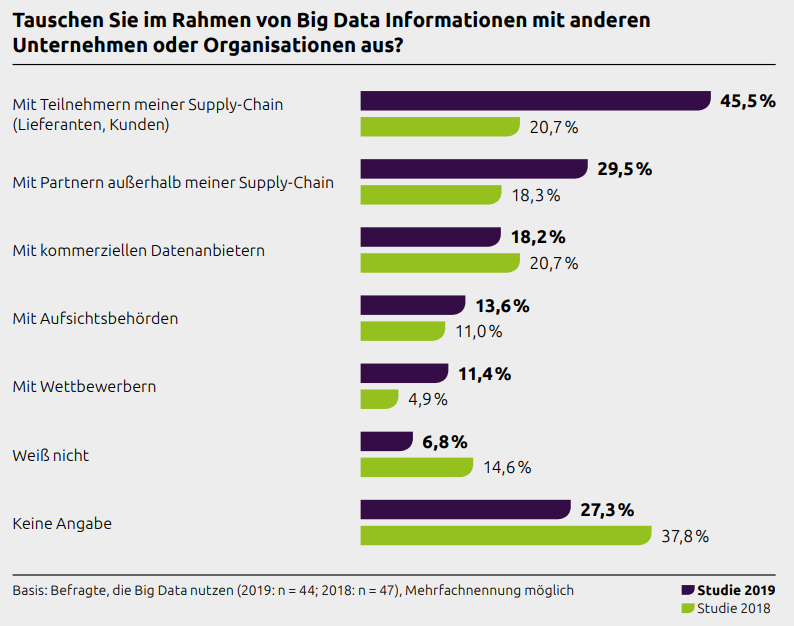
\includegraphics[width=\textwidth]{big_data.png}
    \caption{Big Data Informationsaustausch vor und nach DSGVO-Pflicht}
\end{figure}
\end{center}

Die Quote derer, welche mit externen Partnern außerhalb der Supply-Chain, Daten ausgetauscht haben, ist um 10 Prozentpunkte gestiegen. Ebenfalls einen starken Anstieg nach der DSGVO Umsetzungsfrist hat der Datenaustausch mit Wettbewerbern. Der Anteil der Unternehmen, welcher Daten mit Partnern austauscht hat sich mehr als verdoppelt.

\subsection{IT-Trends Analyse}
Das erste Jahr auf der Liste und gleich eines der Meistdiskutierten Themen ist \textbf{DSGVO-Compliance}. Die EU Verordnung musste bereits am 25.Mai 2018 fertig umgesetzt worden sein, jedoch haben erst rund die Hälfte aller Befragten die DSGVO umgesetzt hat, wobei etwas mehr als ein viertel noch an der Umsetzung arbeitet.

Datenschutzfreundliche Softwareentwicklung und Integration von Datenschutz in die IT-Systeme, welches unter dem Begriff \textbf{Privacy by design} zusammengefasst wird, liegt in der Studie auf Platz, gleich hinter DSGVO-Compliance. 

Dies bewirkt, dass bereits bei der ersten Phase bei einer Softwareentwicklung die DSGVO integriert und mitgedacht werden muss. Zudem müssen jetzt nun auch Sicherheitsfachleute für diesen neuen Fall in den Entwicklungsprozess miteinbezogen werden, was nur jedem sechsten Unternehmen gelungen ist. Rund 13.5 Prozent planen erst, dieses Prozess noch in die Entwicklung zu integrieren.

\section{Datenschutz in EMS}
EMS muss personenbezogene Daten speichern, diese werden jedoch zu keinem Zeitpunkt weiterverarbeitet und weitergeben. Diese Daten werden ausschließlich zu internen Prozessabwicklungen benötigt wie zum Beispiel dem
Anmeldesystem (Kapitel 5). 

\subsection{AWS Datenschutzgrundverordnung}
AWS bietet eine eigene DSGVO Compliance Abteilung\footcite{aws-dsgvo}. Amazon Web Services bieten eine übersichtliche Tabelle\footcite{AWS-DSGVO-Tabelle}, welche angebotenen Dienste genau eine Verschlüsselung, Löschung und 
genaue Überwachung der Daten bieten. Als Beispiel wird hier ein für EMS relevanter Service, AWS EC2, genauer hinsichtlich DSGVO Konformität beschrieben.

Amazon Elastic Compute Cloud (Amazon EC2), bietet vom Anbieter selbst aus eine Verschlüsselung, Löschung und auch Überwachung der Daten\footcite{aws-ec2-dsgvo-alles}. Eine der wichtigsten Tools zur generellen Sicherung von Daten ist es, diese zu
Verschlüsseln. Bei diesem Service, auf welchem das Backend von EMS läuft, ist auch in der gratis Variante eine Verschlüsselung der virtuellen Festplatte geboten. Dies kann man bei der Erstellung einer EC2 Instanz auswählen
(Kapitel 1.3.3, Abb. 1.7). Das sicherste Verschlüsselungsverfahren was auf diesem Service oder generell angeboten wird ist AES256\footcite{aes256}. AES steht für \textbf{Advanced Encryption Standardnpg} und die Zahl nach AES, in dem
Fall hier 256, steht für die Schlüsselänge in Bit. Es ist eines der sichersten Verschlüsselungsverfahren was es Stand bei Verfassung dieser Schrift gab. Es ist von der NSA als sicher genug zur Verschlüsselung von als Top-Secret
eingstuften Dokumenten ausgezeichnet.
Eine EC2 Instanz kann auf zwei verschiedene Arten verschlüsselt werden:

\begin{enumerate}
	\item mit \textbf{disk encryption}
	\item mit \textbf{file-system-level encryption}
\end{enumerate}

Diese zwei Arten unterscheiden sich in einem Grundlegend Punkt. Die erste Methode operiert auf einem Level unter dem Dateisystem und verschlüsselt einen gesamten Block einer Disk oder die ganze Disk. Die zweite Variante
verschlüsselt eine Datei oder einen Ordner in dem Dateisystem direkt. Also disk encryption ist zwar sicherer, dafür ist die zweite Methode kompatibel mit anderen Betriebssystemen.

In EMS wird all dies aber nicht benötigt. Auf der EC2 Instanz läuft das Background, der Node.js/Express Server, mit welchem die App kommuniziert und Funktionen aufruft. Auf der EC2 Instanz werden keine Datenschutzrechtlich
relevanten Daten gespeichert. Diese Funktionen erhalten entweder pseudonymisierten Kürzel oder komplett nicht personenbezogene Daten als Funktionsparameter mit und machen bei Bedarf eine Abfrage auf die MongoDB Datenbank,
welche den Klarnamen eines Benutzers gespeichert hat. Mehr dazu bei Kapiteln 8.1.5 und 8.1.6.

Personenbezogene Daten werden nur einmal zur Anlegung eines neuen Benutzers benötigt. Hier müssen alle in folgender Abbildung gezeigten Felder mit den entsprechenden Daten gefüllt werden um einen neuen Benutzer, einen Promoter, anzulegen.
\begin{center}
	\begin{figure}[h]
		\centering
		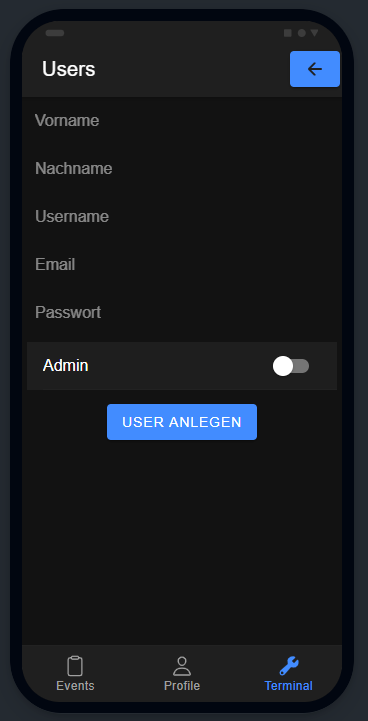
\includegraphics[width=\textwidth]{benutzer_anlegen.png}
		\caption{Benutzerinformationen}
	\end{figure}
\end{center}

%\footnote{https://aws.amazon.com/de/compliance/gdpr-center/}
%\footnote{https://aws.amazon.com/de/compliance/data-privacy/service-capabilities/}
%\footnote{https://aws.amazon.com/de/blogs/security/how-to-protect-data-at-rest-with-amazon-ec2-instance-store-encryption/}
%\footnote{https://en.wikipedia.org/wiki/Advanced_Encryption_Standard}
\newpage